%Esto es un comentario

%Para compilar latex, instalar: texlive-full y después localizarse en el
%directorio de tu archivo latex y dar la orden: pdflatex
%Por ejemplo para este documento: pdflatex prope2020.tex
%En caso de error ingresar: q

%Un lugar para encontrar símbolos matematicos: http://detexify.kirelabs.org/

\documentclass[11pt]{article} %beamer/book/letter

%paquetes a usar
\usepackage[spanish]{babel} %Poner algunas palabras reservadas en español
\usepackage[utf8]{inputenc} %Para aceptar acentos y ñ
\usepackage{authblk} %Poner instituto en la portada
%Paquetes para símbolos matematicos
\usepackage{amsmath}
\usepackage{amssymb}
\usepackage[]{algorithm2e} %Paquete para algoritmos

%Otros paquetes
\usepackage{wasysym}
\usepackage{graphicx}
\usepackage{float}
\usepackage{marvosym}


%Aspectos de la portada
\title{Propedéutico 2020 \\ \LaTeX}
\author{Victor Zamora Gutiérrez \\ Karla Socorro García Alcántara \\
  Emiliano Galeana Araujo}
\affil{Facultad de ciencias, UNAM}
\date{\today}

\begin{document}

%Orden para crear la portada
\maketitle

\section{Aspectos básicos}

Para generar un \texttt{PDF} ingresar en terminal: \texttt{pdflatex
  NombreArchivo.tex}\\

Para generar portada: \verb!\maketitle!\\
Para salto de línea: \verb!\\!\\
Para \textbf{negritas}: \verb!\textbf{texto}!\\
Para \textit{itlaicas}: \verb!\textit{texto}!\\
Para \texttt{máquina de escribir}: \verb!\texttt{texto}!\\

\section{EMACS \Heart}
C-c C-c\\
\begin{figure}[H] % float
  \begin{center}
    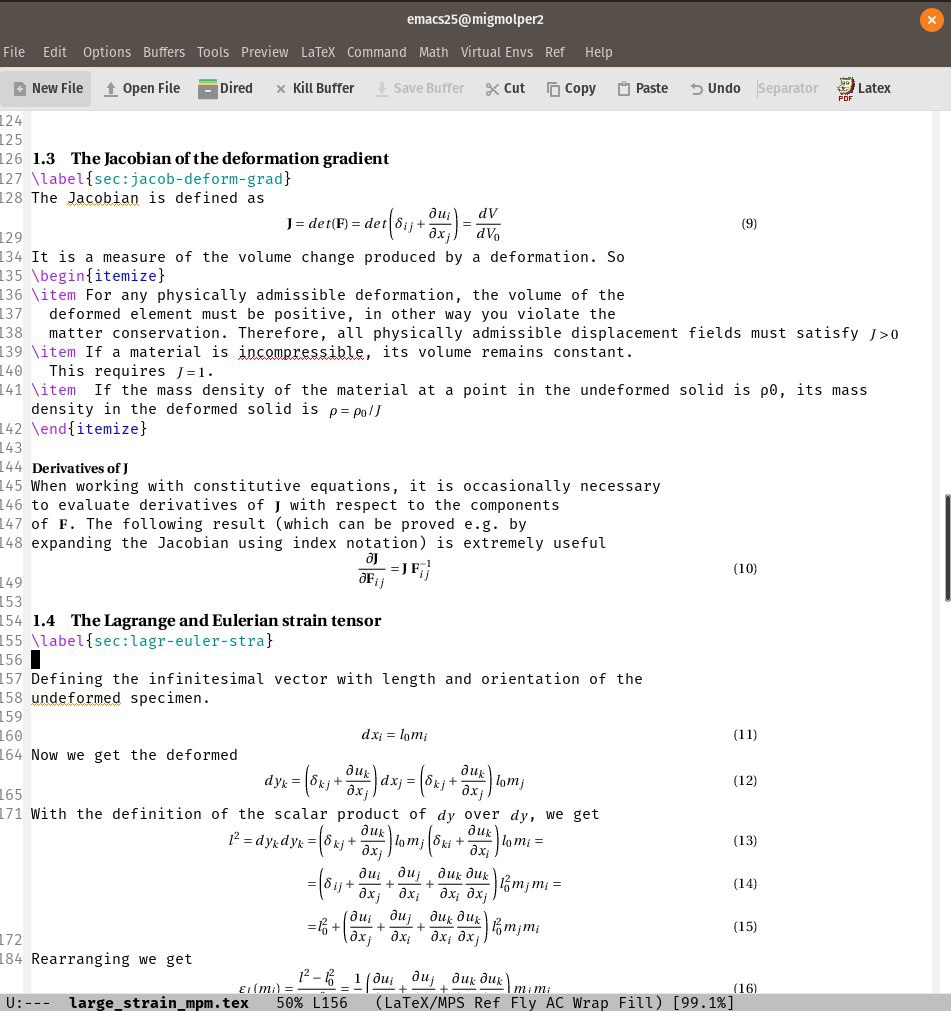
\includegraphics[width=450pt]{./emacs-LaTeX-1.jpg}  
    \caption{Emacs ft. \LaTeX \smiley}
  \end{center}
\end{figure}

\section{Secciones, capítulos, etc}

En caso de los ambientes \verb!article! o bien \verb!report!, pueden definir:
\begin{description}
\item[Sección] Utilizar comando \verb!\section{Nombre_sección}!
\item[Subsección] Utilizar comando \verb!\subsection{Nombre_subsección}!
\end{description}

\subsection{Subsección}
En el caso del ambiente \verb!book!, pueden definir capítulos:\\
Utilizar el comando \verb!\chapter{Nombre_capítulo}!

\section{Listas...}
\subsection{Enumeraciones}
Para crear una lista enumerada utilizar el ambiente \texttt{itemize}.\\
Por ejemplo la siguiente lista:
\begin{enumerate}
\item H
\item O
\item L
\item A
\end{enumerate}
Se escribe en latex como:
\begin{verbatim}
  \begin{enumerate}
  \item H
  \item O
  \item L
  \item A
  \end{enumerate}
\end{verbatim}

\subsection{Sin enueraciones}
Para listas no enumeradas:
\begin{itemize}
\item H
\item O
\item L
\item A
\end{itemize}
Se escribe en latex como:
\begin{verbatim}
  \begin{itemize}
  \item H
  \item O
  \item L
  \item A
  \end{itemize}
\end{verbatim}

\section{Ambiente matemático}
El ambiente matemático se puede poner de dos formas:

\begin{itemize}
\item \verb!$expresionMatematica$!
\item \verb!\[expresionMatematica\]!
\end{itemize}

Ejemplo\\
$ax^2+bx+c \to$ \verb!$ax^2+bx+c$!
\[ax^2+bx+c \to\] \verb!\[ax^2+bx+c\]!

\section{Símbolos lógicos}
Para utilizar símbolos lógicos deben ponerlos en ambiente matemático.
\begin{itemize}
  
\item Conectivos:
  
  \begin{itemize}
  \item Negación ($\lnot$): \verb!\lnot!
  \item Conjunción ($\land$): \verb!\land!
  \item Disyunción ($\lor$): \verb!\lor!
  \item Implicación ($\to$): \verb!\to!
  \item Doble condicional ($\leftrightarrow$): \verb!\leftrightarrow!
  \item Disyunción exclusiva ($\not\equiv$): \verb!\not\equiv!
  \item Conjunción negada ($\uparrow$): \verb!\uparrow!
  \item Disyunción negada ($\downarrow$): \verb!\downarrow!
  \end{itemize}
  
\item Cuantificadores:
  
  \begin{itemize}
  \item Universal ($\forall$): \verb!\forall!
  \item Existencial ($\exists$): \verb!\exists!
  \end{itemize}
  
\item Universo de discurso ($\mathcal{U}$): \verb!\mathcal{U}!
  
\item Lenguaje ($\mathcal{L}$): \verb!\mathcal{L}!
  
\item Derivación semántica ($\vDash$): \verb!\vDash!
  
\item Derivación sintactica ($\vdash$): \verb!\vdash!

\item Relaciones:
  \begin{itemize}
  \item Relación de igualdad ($=$): \verb!=!
  \item Relación menor estricta ($<$): \verb!<!
  \item Relación menor o igual ($\leq$): \verb!\leq!
  \item Relación mayor estricta ($>$): \verb!>!
  \item Relación mayor o igual ($\geq$): \verb!\geq!
  \end{itemize}
  
\end{itemize}

\section{Tablas}

\begin{table}[H]
  \centering
  \begin{tabular}{| c | c || c|}
    \hline
    P & Q  & P$\rightarrow$Q \\ \hline
    0 & 0 & 1 \\ \hline
    0 & 1 & 1 \\ \hline          
    1 & 0 & 0 \\ \hline
    1 & 1 & 1 \\ \hline
  \end{tabular}
  \caption{Representación de la implicación.}
  \label{tabla:implicación}
\end{table}

\section{Imágenes}

\begin{figure}[H] % float
  \begin{center}
    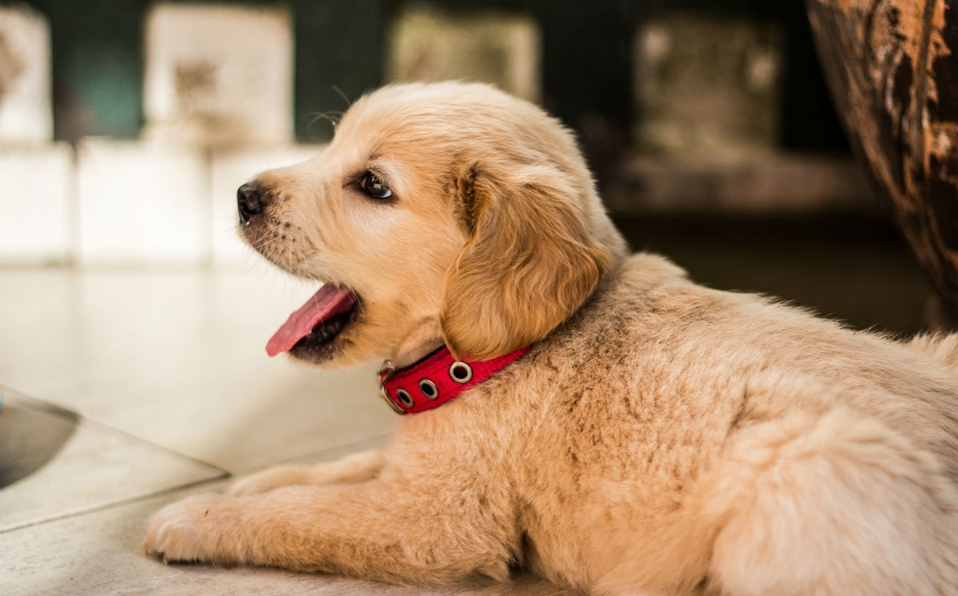
\includegraphics[width=450pt]{./perrito.jpg}
    \caption{Un perritou \smiley}
  \end{center}
\end{figure}

\section{Algoritmos \smiley}
\begin{algorithm}[H]
  \KwData{Entradas}
  \KwResult{Salida del algoritmo}
  print "Hello world''\;
  \While{guardia}{
    instruccion\;
    \eIf{guardia}{
      instruccion true\;
    }{
      instruccion else\;
    }
  }
  \caption{Como escribir algoritmos}
\end{algorithm}

\section{Código}
\dots

\section{Actividad}
En emacs, escribir un archivo de nombre \texttt{#cuenta.tex}, crear una portada,
añadir tu nombre, fecha, facultad. Y cuéntanos algo sobre ti, no tiene que ser
muy extenso... Recuerda usar secciones, subsecciones(OPCIONAL), listas, una
tabla e insertar una imágen de tu animal favorito.\\
En la última sección escribir la fórmula de \textit{La chicharronera}.

\end{document}
